\documentclass[11pt,a4paper]{article}
\usepackage[margin=26mm,top=23mm,bottom=24mm]{geometry}
\usepackage{amsmath,amssymb,booktabs,tikz,xcolor}
\usepackage[colorlinks=true,linkcolor=deepteal,citecolor=deepteal,urlcolor=deepteal]{hyperref}
\definecolor{deepteal}{RGB}{20,91,89}
\definecolor{clay}{RGB}{156,73,50}
\hypersetup{pdftitle={Short Dehn twists at distances five and six on the closed genus-two surface},
 pdfsubject={Explicit curve pairs, a counterexample, and reproducible distance checks}}
\newtheorem{theorem}{Theorem}
\newtheorem{lemma}[theorem]{Lemma}
\newtheorem{corollary}[theorem]{Corollary}
\newcommand{\proof}{\par\noindent\textit{Proof.}\enspace}
\newcommand{\qed}{\hfill\(\square\)\par}
\newcommand{\C}{\mathcal C}
\newcommand{\dist}{\operatorname{dist}}
\newcommand{\diam}{\operatorname{diam}}
\newcommand{\ttcode}[1]{\texttt{\detokenize{#1}}}
\setlength{\parskip}{3.5pt plus 1pt minus .5pt}
\setlength{\parindent}{1.1em}
\setlength{\emergencystretch}{1.2em}
\raggedbottom
\begin{document}
\begin{center}
{\LARGE\bfseries Short Dehn twists at distances five and six\\[3pt]
on the closed genus-two surface\par}
\vspace{9pt}
{\small Research manuscript \(\,\cdot\,\) 25 November 2026}
\end{center}

\begin{abstract}
For the twelve-intersection distance-four pair \((a,b)\) in Figure 18 of
Mahanta's distance-five preprint, we determine \(d(a,T_b^k a)\) for every
integer \(k\). Its value is five for \(|k|=1\) and six for \(|k|\ge2\).
We give two more genus-two diagrams. A fourteen-intersection seed produces
a distance-six pair with 196 intersections after a single twist. A
complete enumeration shows that every distance-four seed with twelve or
thirteen intersections gives distance five after a single twist. Thus
fourteen is the least possible seed intersection for this construction.
Minimality is sufficient in genus two, as conjectured in version 2 of
Mahanta's preprint, and the thirteen-intersection examples disprove the
necessity conjectured in version 3. The proof combines efficient
geodesics, annular projection, and reproducible finite computations.
\end{abstract}

\section{The small-power problem}
Let \(S_g\) be a closed, connected, orientable surface of genus \(g\ge2\).
The vertices of \(\C(S_g)\) are isotopy classes of essential simple closed
curves. Distinct vertices share an edge when they admit disjoint
representatives. Write \(d\) for graph distance and \(i\) for the minimum
number of transverse intersections over all representatives.

In a connected graph of infinite diameter, the first \(n\) edges of a
sufficiently long geodesic give a pair at distance \(n\). For curve
graphs, Masur and Schleimer \cite[proof of Lemma~2.5]{MS} trace the
infinite-diameter argument to Kobayashi \cite[Prop.~2.2]{K}. Masur and
Minsky state the result explicitly \cite[Thm.~1.1]{MM1}. Schleimer
constructs the next distance inductively \cite[proof of Prop.~3.1]{S}.
Ido, Jang and Kobayashi give a six-edge geodesic on taking \(n=6\)
\cite[Construction~4.6 and Assertion~4.7]{IJK}. Aougab and Taylor's
large Dehn twists also produce length six \cite[\S5, Lemma~5.1]{AT}.
For a specified pair and a small twist, a six-edge walk leaves every
possible shortcut to exclude. Each vertex has infinitely many neighbors.

Write \(D_k(a,b)=d(a,T_b^k a)\). Mahanta and Palaparthi prove that
\(D_1=4\) whenever \(d(a,b)=3\) \cite[Theorem 2]{MP}. For a distance-four
input, Mahanta bounds \(D_1\) between four and six. Her stacking criterion
detects four-edge paths, and her Theorem 2 reduces the test when there
are no complementary hexagons. Figure 18 has hexagons. A separate argument
gives \(D_1=5\) with 144 endpoint crossings. Question 1 asks which positive
powers give six \cite[Lemma 9, Theorem 2 and \S6]{M}.
Table~\ref{tab:short} records our answers for three marked inputs. Write
\(i_{\min}(2,6)\) for the least intersection over all distance-six pairs on \(S_2\).

\begin{table}[h]
\centering
\begin{tabular}{lrrrl}
\toprule
Seed & \(i(a,b)\) & \(|k|\) & \(i(a,T_b^k a)\) & \(D_k(a,b)\)\\
\midrule
Figure 18 & 12 & 1 & 144 & 5 \quad\cite[\S6]{M}\\
Figure 18 & 12 & 2 & 288 & 6\\
Figure 18 & 12 & 3 & 432 & 6\\
Thirteen crossings & 13 & 1 & 169 & 5\\
Fourteen crossings & 14 & 1 & 196 & 6\\
\bottomrule
\end{tabular}
\caption{Each seed has distance four. The same sign convention is used
throughout.}\label{tab:short}
\end{table}

\clearpage
\section{Three marked pairs of curves}\label{sec:input}
Orient \(a,b\) and number their \(N\) crossings in cyclic order on \(a\).
Record the crossing labels encountered on \(b\), giving a positive sign
when \(b\) leaves the crossing on the chosen positive side of \(a\).
This is a signed cyclic permutation. To reconstruct its surface, make one
four-valent vertex per label and connect the consecutive labels on each
curve. Give the four incident half-edges the cyclic order prescribed by
the sign, thicken the graph, and cap every boundary circle by a disk.
The two cycles through the graph give the marked pair.

\begin{align*}
P_{12}&=(1,-8,-3,-10,5,6,7,-2,-9,-4,11,12),\\
P_{13}&=(1,-8,-3,-9,-4,11,13,2,7,6,5,10,12),\\
P_{14}&=(1,-9,-3,-11,-5,-6,-7,-8,-2,-10,-4,12,13,14).
\end{align*}

The cyclic orders of \(P_{12}\) can be checked directly against the labeled
polygons in Figures 22--27 of \cite{M}. For example, the boundary of
\(H_1\) reads \(1,8,9,2,1,12\), up to cyclic order and reversal. The
nine pictured faces determine the remaining rectangle with cyclic labels
\(4,5,10,11\). The text in the example lists \(10,9,4,5\) for
this omitted face. We use the labeled faces and the curves in the figure.

For \(P_N\) the face cycles consist of \(N-6\) rectangles and four
hexagons. Thus \(V=N\), \(E=2N\), \(F=N-2\), and \(V-E+F=-2\).
The capped surface is \(S_2\). Its complementary disks have at least
four sides, so the marked curves are in minimal position by the bigon
criterion. In particular, the subscript gives their geometric intersection
number.

\paragraph{How the extra seeds were found.}
Cut \(P_{12}\) along \(a\) and replace each of the six parallel families
of \(b\)-arcs by a single arc. Give the six arcs positive integer
multiplicities. Whenever the boundary circles have equal numbers of
ends, reglue their ends in opposite boundary order with a cyclic offset.
Keep the resulting \(b\) when it has one component. In the edge order
of \ttcode{generate_seeds.py}, \(P_{13}\) has widths \((1,1,4,4,2,1)\)
and offset 11. For \(P_{14}\) the widths are \((1,2,3,4,3,1)\) and the
offset is 13. Glenn, Menasco, Morrell and Morse tabulated distance-four
seed weights at these intersection numbers \cite[\S6]{GMMM}. Here we
compute the distances of the twisted images.

\begin{theorem}\label{thm:main}
Let \((a,b)\) be the marked pair specified by \(P_N\).
\begin{enumerate}
\item For \(P_{12}\), \(D_0=0\), \(D_1=D_{-1}=5\), and
\(D_k=6\) for every \(|k|\ge2\).
\item For \(P_{13}\), \(d(a,b)=4\) and \(D_1=5\).
\item For \(P_{14}\), \(d(a,b)=4\) and \(D_1=6\). In particular
\(i_{\min}(2,6)\le196\).
\end{enumerate}
\end{theorem}

\proof Section~\ref{sec:finite} proves completeness of the computation
reported in Section~\ref{sec:results}. It gives distance four for all
three seeds and the small powers in Table~\ref{tab:short}.
Lemma~\ref{lem:fold} gives \(D_k=6\) for \(|k|\ge4\).
Applying the inverse twist and using symmetry of distance gives
\(D_{-k}=D_k\). The twist intersection formula gives
\(i(a,T_b^k a)=|k|\,i(a,b)^2\) \cite[\S4]{AT}. \qed

\begin{corollary}\label{cor:min}
A distance-four pair on \(S_2\) can give distance five after one twist
even when it has more crossings than another distance-four pair.
\end{corollary}
\proof Use \(P_{13}\) for the unit twist. The distance-four seed \(P_{12}\)
has fewer crossings. This contradicts the necessary minimality condition
conjectured in the introduction of \cite[version 3]{M}. The comparison
only uses \(12<13\). \qed

\clearpage
\section{A uniform bound from the annular cover}
Write \(Y\) for the compactified annular cover associated with a curve
\(c\). For a curve intersecting \(c\), let \(\pi_c\) be its collection of
spanning lifts in the annular arc graph. We use
\(d_c(x,y)=\diam(\pi_c(x)\cup\pi_c(y))\). Two disjoint curves crossing
\(c\) have disjoint spanning lifts, so their union of projections has
diameter at most one. The annular twist formula in
\cite[\S2.4, (2.6)]{MM2} is
\[
 d_c(x,T_c^k x)=|k|+2\qquad(k\ne0,\ i(x,c)>0).
\]
The convention matters for the small powers here. In the same reference
the twist supported directly on the covering annulus moves one chosen
arc by \(|k|\). Equation (2.6) concerns the projections of two curves
on the original surface.

\begin{lemma}\label{lem:fold}
Let \(a=v_0,v_1,\ldots,v_r=c\) be a geodesic in \(\C(S_g)\), where
\(r\ge4\), and set \(F=T_c^k\). If \(|k|\ge2r-4\), then
\(d(a,Fa)=2r-2\).
\end{lemma}
\proof Put \(w=v_{r-1}\). Since \(w\) misses \(c\), the twist fixes
\(w\). Following the original geodesic as far as \(w\), then the twisted
prefix in reverse, gives the path
\[
  v_0,\ v_1,\ldots,v_{r-2},\ w,\ Fv_{r-2},\ldots,Fv_1,\ Fv_0 .
\]
Its length is \(2r-2\). To obtain the reverse inequality, consider any
path from \(a\) to \(Fa\). If every vertex intersects \(c\), choose
spanning lifts at the endpoints attaining their projection distance and
an arbitrary spanning lift at each intervening vertex. Consecutive lifts
are at distance at most one, hence the path has length at least
\(|k|+2\ge2r-2\).

Otherwise some vertex \(z\) satisfies \(d(z,c)\le1\). Both endpoints
have distance \(r\) from \(c\) because \(F\) fixes \(c\) and acts
isometrically. The triangle inequality gives \(d(a,z)\ge r-1\) and
\(d(z,Fa)\ge r-1\). Adding the two bounds proves the lemma. \qed

\begin{figure}[h]
\centering
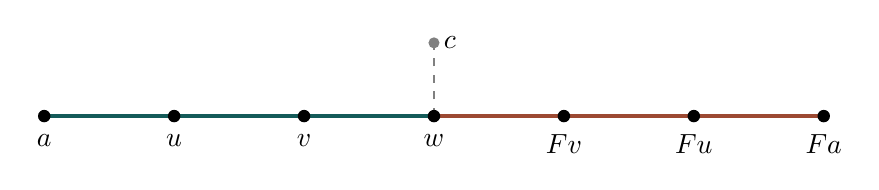
\begin{tikzpicture}[x=1.65cm,y=.93cm]
\draw[very thick,deepteal] (0,0)--(3,0);
\draw[very thick,clay] (3,0)--(6,0);
\draw[dashed,gray] (3,0)--(3,1);
\foreach \i/\name in {0/a,1/u,2/v,3/w,4/Fv,5/Fu,6/Fa}
  {\fill (\i,0) circle (2.25pt); \node[below=3pt] at (\i,0) {\(\name\)};}
\fill[gray] (3,1) circle (2pt);
\node[right] at (3,1) {\(c\)};
\end{tikzpicture}
\caption{The six-edge walk for \(r=4\). It turns at \(w\), one edge
short of the twist core. The core itself is outside the displayed walk.}
\end{figure}

The same proof before imposing the threshold gives, for \(k\ne0\),
\[
 \min\{|k|+2,\,2r-2\}\ \le\ d(a,T_c^k a)\ \le\ 2r-2 .
\]
For \(r=4\) and powers two and three the annular lower bounds are four
and five. A path of length five is compatible with either bound. This
is the precise gap that the finite test must close. At power one there
can actually be a shorter route, as \(P_{12}\) and \(P_{13}\) show.

Yoshizawa's nested high-power example gives distance six from a disk
set \cite[p.~1000]{Y}. For individual curves, Mahanta explicitly derives
eventual distance six for every distance-four seed in the thesis
\cite[pp.~47--48]{MT}. Lemma~\ref{lem:fold} gives the uniform sufficient
power four in this case.

\clearpage
\section{A finite, exhaustive short-path test}\label{sec:finite}
Fix two vertices \(x,y\) given in minimal position. For a budget \(m\ge2\)
the checker decides the predicate \(d(x,y)\le m\). Its terminal test asks
whether the curves \emph{fill}, meaning that their complement is a union
of disks.

\paragraph{The terminal calculation.}
For an intersecting pair with \(N\) crossings, the connected ribbon
neighborhood \(R\) has Euler characteristic \(-N\). If its ribbon
permutation has \(f\) boundary cycles, its genus is
\[
                         h=(2+N-f)/2.
\]
For complement components of genera \(g_j\) and boundary counts \(b_j\),
Euler characteristic gives
\(g-h=\sum_j(g_j+b_j-1)\). Each summand is nonnegative and vanishes
exactly for a disk. Thus \(h=g\) is equivalent to filling. A
nonfilling intersecting pair on the closed surface has an essential
curve disjoint from both, and conversely. It therefore has distance at
most two exactly when \(h<g\). A zero-crossing diagram satisfies the
predicate immediately. This explains the entire budget-two test.

\paragraph{Finding possible first moves.}
For a filling pair, cut \(S_g\) along \(x\) and treat its boundary
circles as ideal vertices. The segments of \(y\) become properly
embedded arcs that cut the surface into polygons. Collapse parallel
bands and add fan diagonals in the remaining polygons to obtain an ideal
triangulation. In genus two it has six edges and four triangles, counting
all components when the cut separates. If the true distance is
\(\ell\ge3\), the efficient-geodesic theorem \cite[Theorem 1.1]{BMM}
supplies a geodesic whose first neighbor meets each of these reference
arcs at most \(\ell-1\) times. When every edge is represented by a
segment of \(y\), Proposition 3.7 of \cite{BMM} gives the simultaneous
bound \(\ell-2\). Only existence of one suitable first move is needed.

Enumerate the six integer edge weights between zero and \(m-1\), or
between zero and \(m-2\) in the latter case. In a triangle with side
weights \(u,v,w\), disjoint normal arcs exist precisely when the triangle
inequalities hold and \(u+v+w\) is even. The number joining the first
two sides is \((u+v-w)/2\). The other two counts follow cyclically.
These counts uniquely determine the matching inside the triangle.
Across a glued edge match the strands in reversed boundary order.
Discard empty and disconnected systems. A nonempty connected normal
curve in this ideal triangulation is essential or peripheral on the cut
surface. A peripheral curve represents \(x\) after regluing and merely
repeats the current vertex.

\paragraph{Recursion and correctness.}
Trace a candidate \(z\) across the original parallel bands and record
its signed crossing order with \(y\). The normal representative has no
bigon with a side of the triangulation. The parallel copies in a band
can be placed as product arcs. A hypothetical bigon with \(y\) disjoint
from \(x\) would give a bigon with one of those arcs. If the bigon meets
\(x\), an outermost arc on its \(y\)-side gives a bigon between \(x\)
and \(y\), since \(x\) misses \(z\). Thus the recursive input is minimal.
Return true if some such \(z\) satisfies \(d(z,y)\le m-1\). Induction on
\(m\) now proves soundness and completeness. A positive branch
prepends a disjointness step (or deletes a repetition). For completeness,
a shortest path of length \(\ell\le m\) for a filling input has a first
move among the enumerated weights, leaving a tail of length \(\ell-1\).

\clearpage
\section{Coordinates, witnesses and computation}\label{sec:results}
The checker constructs \(T_b^k a\) in a collar of \(b\). For positive
\(k\), take circumference \(4N\) and put the \(j\)-th strand of \(a\)
at column \(4j\), \(0\le j<N\), in cyclic order along \(b\). Push the
second copy of \(a\) consistently to one side. Depending on its
orientation its strand starts at \(4j+1\) or \(4j-1\), sweeps through
\(k\) turns from the bottom of the collar to the top, and rejoins its
parallel copy outside. Every fixed and moving strand pair intersects
\(k\) times. Order these crossings first along the fixed curve, then
along the moving curve, reversing the height order for a
downward-traversed strand. The product of the two strand signs gives
the crossing sign up to global orientation. The resulting diagram has
\(kN^2\) crossings, the geometric twist intersection number, so it is
minimal.

\begin{center}
\small
\begin{tabular}{lrrrrr}
\toprule
Input & Target distance & \(m=5\) & \(m=4\) & \(m=3\) & \(m=2\)\\
\midrule
\(P_{12},P_{13},P_{14}\), each seed &4&--&--&1&6\\
\(P_{12}\), one twist &5&--&1&30&180\\
\(P_{13}\), one twist &5&--&1&30&180\\
\(P_{12}\), two twists &6&1&80&2,336&14,016\\
\(P_{12}\), three twists &6&1&80&2,336&14,016\\
\(P_{14}\), one twist &6&1&80&2,336&14,016\\
\bottomrule
\end{tabular}
\end{center}
The counts are recursive calls made while rejecting a path one edge shorter
than the target. They count occurrences, so repeated isotopy classes need
not produce distinct entries. In each row every budget-two diagram fills.
The program also accepts at the target budget. As a check on the terminal
calculation, its audit mode compares the full multiset of face lengths
obtained from two permutations at every nonempty input. One uses two
darts per cut segment. The other works on the original four-valent
graph, reversing an edge and then rotating around the arrival crossing.

\paragraph{A short positive witness for the counterexample.}
For the unit twist of \(P_{13}\), successive first moves have normal
weights
\[
   (0,0,0,1,1,0),\quad (1,1,0,0,0,0),\quad(1,1,0,0,0,0).
\]
Number edges by first occurrence in the checker's ordered list of
triangle sides, recomputed at each stage. After three moves the pair has
four crossings and its regular neighborhood has genus one. A common
disjoint curve supplies the final two steps. At budget four the 180
terminal diagrams all have neighborhood genus two. These two facts give
the equality five.

\paragraph{Reproduction.}
Run \ttcode{python verify_distance_six.py --audit} using Python 3.9 or
later. The supplement contains the code, the audit transcript and the
positive coordinates for these cases and the nested twist in Section~6. Running
\ttcode{python certificates.py} reconstructs these coordinates from the
seed permutations. Only the Python standard library is required for the
distance computation.

\clearpage
\section{Prescribing a distance on one surface}
For an explicit starting path, take four unit squares. Glue right edges
to left edges by the cycle \((1\,2\,3\,4)\) and top edges to bottom edges
by \((1\,2\,4\,3)\), all by translations. The corners form two classes.
Thus \(V-E+F=2-8+4=-2\). The horizontal and vertical midlines concatenate
to simple closed curves \(h\) and \(v\).

\begin{center}
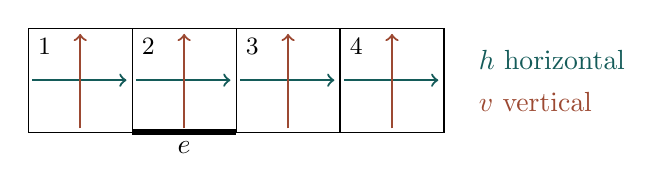
\begin{tikzpicture}[scale=.8]
\foreach \i in {0,1,2,3}{
 \draw (\i*1.65,0) rectangle ++(1.65,1.65);
 \draw[deepteal,thick,->] (\i*1.65+.06,.825)--++(1.50,0);
 \draw[clay,thick,->] (\i*1.65+.825,.06)--++(0,1.50);
 \node[below right] at (\i*1.65,1.65) {\small\the\numexpr\i+1\relax};}
\draw[line width=2pt] (1.65,0)--(3.30,0);
\node[below] at (2.475,0) {\(e\)};
\node[right,deepteal] at (7.0,1.15) {\(h\) horizontal};
\node[right,clay] at (7.0,.48) {\(v\) vertical};
\end{tikzpicture}
\end{center}
The two components of the complement of \(h\cup v\) are disks about
the corner classes, so \(h,v\) fill. The bottom edge \(e\) of square
2 has coincident endpoints. Smoothing there gives a simple loop
disjoint from \(h\) and intersecting \(v\) once. The boundary \(s\)
of a small regular neighborhood of \(e\cup v\) bounds a one-holed torus
and is essential in \(S_2\). Thus \(h,e,s,v\) is a length-three
geodesic. For \(P=T_v\), the sequence
\(h,e,s,Pe,Ph\) is a path since \(Ps=s\). Its endpoints are four
apart by \cite[Theorem 2]{MP}. For example, the vertices \(h\) and
\(T_{Ph}^{\,4}h\) are six apart by Lemma~\ref{lem:fold}. This example
has a proof using only the stated surface theorems.

Starting at length four, apply Lemma~\ref{lem:fold} with \(k=2r-4\).
The successive lengths are \(4,6,10,18,34,\ldots\). Given \(n\ge0\),
choose the first such path of length at least \(n\). Its first vertex
and its \(n\)-th vertex, counting from zero, have distance \(n\).
A shorter path to the \(n\)-th vertex would shorten the whole path.
The supplement prints the two vertices as twist words when called with
\ttcode{--distance N}. For a worked example put
\[
       F_1=T_{Ph}^{\,4},\qquad F_2=T_{F_1h}^{\,8}.
\]
On the length-six path the third vertex after \(h\) is \(Pe\).
On the length-ten path the seventh vertex after \(h\) is its image under
\(F_2\). Hence \(d(h,F_2(Pe))=7\).

\paragraph{The nested unit twist.}
Mahanta's thesis \cite[\S1.2, p.~6]{MT} suggests considering
\(d(a,T_{T_c a}a)\) for \(d(a,c)=3\). On these four squares the signed
word of \((h,v)\) is \((1,2,4,3)\). Applying the collar construction
twice gives 256 crossings and \(d(h,T_{T_v h}h)=5\). At budget four the
search rejects all 1,718 terminal diagrams. At budget five the three
successive weight vectors are
\((0,0,0,1,1,1),(1,1,0,0,0,0),(0,1,1,0,1,1)\).
The last pair intersects once and lies in a one-holed torus. This
evaluates the formula on one distance-three input.

\clearpage
\section{The smallest seed for a single twist on \texorpdfstring{\(S_2\)}{S2}}\label{sec:census}
Mahanta's version 2 proposes that a distance-four pair of minimum
intersection gives distance five after one twist. The attached
version 3 reverses this implication. The thesis asks the version 2
question again \cite[p.~2 in each version]{M}\cite[\S1.2, Question~4]{MT}.
On \(S_2\), the minimum is twelve \cite[Theorem~1.6]{GMMM}.

\begin{theorem}\label{thm:census}
For every ordered pair \((a,b)\) on \(S_2\) with \(d(a,b)=4\) and
\(i(a,b)\in\{12,13\}\), one has \(d(a,T_ba)=5\). The least
\(i(a,b)\) for a distance-four pair satisfying \(d(a,T_ba)=6\) is
fourteen. The least intersection of the resulting distance-six endpoints
in this single-twist construction is \(14^2=196\).
\end{theorem}

\proof We show how to exhaust the input diagrams. Cut \(S_2\) along
\(a\), obtaining either a twice-bordered torus or two once-bordered tori.
The arcs of \(b\) are essential by the bigon criterion. They cut the
surface into disks because \(d(a,b)=4\). Collapse parallel families,
mark the two boundary circles as ideal vertices and complete the arc
system to an ideal triangulation by adding polygon diagonals. Euler
characteristic and the fact that there are two sides per edge give four
triangles and six edges, including in the disconnected case.

Label the twelve triangle sides in four cyclic triples with rotation
\(\rho\). An orientation-reversing edge gluing is specified by a
fixed-point-free involution \(\tau\) of these sides. Ideal vertices are the
cycles of \(\rho\tau\). The program enumerates all \(11!!=10{,}395\)
pairings. Exactly 4,563 have two vertex cycles. They give six types
up to oriented isomorphism. As a check, applying the
\(4!\,3^4=1{,}944\) triangle relabelings to these six representatives
recovers exactly the original 4,563 pairings in disjoint orbits.

For each type, put nonnegative integer widths summing to \(N\) on the
six edges. On each boundary, read the endpoints of the parallel bundles
in its cyclic order. If both circles have \(N\) endpoints, glue them
in reversed boundary order with each of the \(N\) cyclic offsets. This
includes every gluing up to a twist about \(a\), which preserves the
marked pair up to homeomorphism. Retain a single connected \(b\), and
require \(N-2\) faces and no bigon. Enumerate cyclic starting points and
direction reversals on both curves and allow a global change of crossing
sign to identify diagrams. For filling pairs these operations just
relabel the signed ribbon graph or reverse surface orientation. Orientation
reversal preserves \(D_1\) since \(D_{-1}=D_1\). The roles of \(a\) and
\(b\) stay ordered.

\begin{center}\small
\begin{tabular}{rrrr}
\toprule
\(N\) & Ordered filling classes & Classes at \(d=4\) & Among these, \(D_1=5\)\\
\midrule
12 & 348 & 5 & 5\\
13 & 499 & 11 & 11\\
\bottomrule
\end{tabular}
\end{center}

Applying Section~\ref{sec:finite} gives the table. The supplement's
\ttcode{census_small_seeds.py} lists all sixteen seeds and checks their
twists. Theorem~\ref{thm:main} supplies the fourteen-crossing example.
The twist intersection formula finishes the proof. \qed

Allowing higher powers of the same construction leaves 196 minimal,
since \(|k|\ge2\) gives at least \(2\cdot12^2=288\) endpoint crossings.
For unrestricted pairs, Jin and Menasco's intersection growth inequality
gives \(i_{\min}(2,6)\ge 12\cdot2^{6-4}=48\) \cite[Theorem~1.3]{JM}.
These results give \(48\le i_{\min}(2,6)\le196\). Determining the
unrestricted minimum and classifying the small powers for every
distance-four pair remain separate questions.

\clearpage
\section{Scope of the formal checks}
The Lean file \ttcode{CurveDistance.lean} defines walks with their
length as a type index and defines exact distance by existence and
minimality. Its theorem \ttcode{fold_exact} takes a fixed vertex, an
edge-preserving twist, unit edge bounds for the height \(h(x)=d(x,c)\),
and a coordinate \(p\) with unit edge change when both heights exceed one.
For the surface application take \(p(x)\) to be the distance from a
fixed extremal initial arc to a chosen arc of \(\pi_c(x)\), choosing
the final arc to attain the endpoint diameter. Vertices of height at most
one can be assigned any \(p\). Induction on an arbitrary walk of length
\(m\) proves \(p(y)\le p(x)+m\) or \(h(x)+h(y)\le m+2\).
The file constructs the folded walk and proves it shortest under the
endpoint gap. It also proves the geodesic-prefix theorem. The theorem
\ttcode{finite_search_correct} verifies the induction in
Section~\ref{sec:finite} for an abstract diagram type, given the local
terminal criterion, legality of first moves, and existence of an
efficient first neighbor. Lean 4.8.0 accepts all three proofs with its
standard logical foundations.

\paragraph{Evaluating the concrete examples in Lean.}
The second file, \ttcode{FiniteDiagrams.lean}, implements the collar
construction and the bounded search directly from the three signed
permutations. For the terminal genus it walks the four-valent graph.
Inside a triangle it computes the next strand from a slot's index
and the corner count, independently of the slot-matching tables in
the Python implementation. It generates the weight vectors and both
possible path bounds without importing the Python results. Both
implementations agree on all eight inputs in Section~\ref{sec:results},
the nested unit twist in Section~6, and the reported distances four and
five for all sixteen signed seeds in Section~\ref{sec:census}. The
exhaustive generation of the census inputs runs in Python.
The concrete equalities are checked with \ttcode{native_decide}. Lean's
printed axiom reports identify the additional evaluator dependency
\ttcode{Lean.ofReduceBool}. The generic graph theorems use ordinary
kernel-checked proof terms.

These checks leave a precise mathematical interface. Identifying signed
diagrams with their geometric realizations, interpreting the collar as
a Dehn twist, and supplying the efficient-geodesic and annular projection
facts are justified in the paper and the cited surface theorems. A full
formalization of the curve graph of \(S_2\) would also have to prove
these identifications in Lean.

\clearpage
\begin{thebibliography}{99}\small
\bibitem{AT} T. Aougab and S. J. Taylor.
Small intersection numbers in the curve graph.
\emph{Bull. Lond. Math. Soc.} \textbf{46} (2014), 989--1002.
\href{https://arxiv.org/abs/1310.4711}{arXiv:1310.4711}.
\bibitem{BMM} J. Birman, D. Margalit and W. Menasco.
Efficient geodesics and an effective algorithm for distance in the complex
of curves. \emph{Math. Ann.} \textbf{366} (2016), 1253--1279.
\href{https://arxiv.org/abs/1408.4133}{arXiv:1408.4133}.
\bibitem{GMMM} P. Glenn, W. W. Menasco, K. Morrell and M. Morse.
MICC: A tool for computing short distances in the curve complex.
\emph{J. Symbolic Comput.} \textbf{78} (2017), 115--132. Preprint 2014.
\href{https://arxiv.org/abs/1408.4134}{arXiv:1408.4134}.
\bibitem{IJK} A. Ido, Y. Jang and T. Kobayashi.
Heegaard splittings of distance exactly \(n\).
\emph{Algebr. Geom. Topol.} \textbf{14} (2014), 1395--1411.
\href{https://msp.org/agt/2014/14-3/agt-v14-n3-p06-p.pdf}{Journal article}.
\bibitem{JM} X. Jin and W. W. Menasco. Super efficient geodesics in
the complex of curves. Version 4, 2023.
\href{https://arxiv.org/pdf/2008.09665v4}{arXiv:2008.09665v4}.
\bibitem{K} T. Kobayashi. Heights of simple loops and pseudo-Anosov
homeomorphisms. In \emph{Braids}, Contemp. Math. \textbf{78} (1988),
327--338. \href{https://doi.org/10.1090/conm/078/975087}{Chapter DOI}.
\bibitem{M} K. Mahanta. Distance 5 curves in the curve graph of closed
surfaces. Preprint series \href{https://arxiv.org/pdf/2211.15290v1}{v1
(2022)}, \href{https://arxiv.org/pdf/2211.15290v2}{v2 (March 2023)},
\href{https://arxiv.org/pdf/2211.15290v3}{v3 (August 2023)}.
\href{https://doi.org/10.1142/S179352532650007X}{Journal DOI}.
The conjecture wording cited here is version-specific.
\bibitem{MT} K. Mahanta. \emph{Local Geometry of Curve Graphs of Closed
Surfaces}. Doctoral thesis, Indian Institute of Technology Guwahati.
Title page dated 2023, viva 12 January 2024.
\href{https://gyan.iitg.ac.in/handle/123456789/2544}{Institutional repository}.
\bibitem{MP} K. Mahanta and S. Palaparthi.
Distance 4 curves on closed surfaces of arbitrary genus.
\emph{Topology Appl.} \textbf{314} (2022), 108137.
\href{https://doi.org/10.1016/j.topol.2022.108137}{doi:10.1016/j.topol.2022.108137}.
\bibitem{MM1} H. A. Masur and Y. N. Minsky.
Geometry of the complex of curves I. Hyperbolicity.
\emph{Invent. Math.} \textbf{138} (1999), 103--149.
\href{https://arxiv.org/abs/math/9804098}{arXiv:math/9804098}.
\bibitem{MM2} H. A. Masur and Y. N. Minsky.
Geometry of the complex of curves II. Hierarchical structure.
\emph{Geom. Funct. Anal.} \textbf{10} (2000), 902--974.
\href{https://arxiv.org/abs/math/9807150}{arXiv:math/9807150}.
\bibitem{MS} H. A. Masur and S. Schleimer. The geometry of the disk
complex. \emph{J. Amer. Math. Soc.} \textbf{26} (2013), 1--62.
\href{https://sschleimer.warwick.ac.uk/Maths/2012geom_disk_complex.pdf}{Authors' copy}.
\bibitem{S} S. Schleimer. The end of the curve complex.
\emph{Groups Geom. Dyn.} \textbf{5} (2011), 169--176. Preprint 2006.
\href{https://arxiv.org/abs/math/0608505}{arXiv:math/0608505}.
\bibitem{Y} M. Yoshizawa. High distance Heegaard splittings via Dehn
twists. \emph{Algebr. Geom. Topol.} \textbf{14} (2014), 979--1004.
\href{https://msp.org/agt/2014/14-2/agt-v14-n2-p13-s.pdf}{Journal article}.
\end{thebibliography}
\end{document}
